\documentclass{l4proj}

%Packages
\usepackage{natbib}
\usepackage{graphicx}
\usepackage[normalem]{ulem}
\useunder{\uline}{\ul}{}
\usepackage{pdflscape}

\begin{document}
\title{Augmented Reality Android Gym App}
\author{David Benicek 2073063b}
\date{\today}
\maketitle

\begin{abstract}
Something will go here.
\end{abstract}

\educationalconsent
%
%NOTE: if you include the educationalconsent (above) and your project is graded an A then
%      it may be entered in the CS Hall of Fame
%
\tableofcontents
%==============================================================================

\chapter{Introduction}
\pagenumbering{arabic}
\section{Motivation}
Frequent exercise and a healthy lifestyle have recently become an integral part of the western culture. Indeed, last year in America more people have exercised on a regular basis then ever before \cite{riffkin_so_2015}. As people begin to adopt their new and healthy lifestyle, they are faced with a lack of common consensus on how best to exercises and how to stay safe while experimenting with new movements. It is important to note that a lack of coherent information does not necessarily mean a lack of data but instead a lack of a singular consensus in the midst of conflicting information, fad diets and ill-informed advice. Similar problems plague even the more experienced gym goes as after some time spent following a routine, every individual will begin to experiment diminishing returns and their progress will plateau. There is therefore a need for a singular portal to which both beginners and experienced gym goers alike can refer to for information regarding exercise.  

\section{Aim} \label{sec:aim}
Tackling the entire topic of fitness in one application would be extremely difficult, if not impossible. Due to this, this project is going to seek to add value to users predominantly while they are in the gym. The aim of the end product will be to help users understand how to use gym equipment, suggest a range of exercises that can be carried out on a given piece of equipment and demonstrate how to perform the exercise with correct and safe form. The product will have to be highly portable and usable in any environment. As a result of this, the product is likely to be a mobile application since most individuals poses a phone and bring it with them everywhere they go.

One of the main goals of the product is for it to be responsive to the user's environment and heavily interactive so that the user has an immersive experience. An immersive experience will keep users engaged with the product thought there is a balance to be drawn here. Since the gym is a potentially dangerous environment, the design of the product must make sure that users do not loose track of their surroundings completely. One possible way of striking this balance is through augmented reality (AR). AR would allow the product to provide a somewhat immersive experience by super imposing realistic human models on the device's screen without the need for a completely virtualized reality. Similar applications of AR have been trialed in education, construction, sports and medicine to various degrees of success. A review of literature regarding previous work done with AR can be found in section \ref{sec:litrew}.

\section{Outline}
This document explores the different steps taken in the development of the augmented reality gym app. First, relevant literature is reviewed, informing design decisions and serving as a basis for requirements elicitation. Following is a summary and review of a discussion with the Glasgow University Sports Association (GUSA) which served as a secondary source of requirements for the app. In the implementation stage, each of the three iterations of development are summarised and major milestones and barriers encountered during the process are highlighted. At the end of each iteration, testing is carried out and further requirements and possible improvements are identified. Finally, the document is drawn to a close with an evaluation which addresses to what extend the main objectives of the project were achieved and reflects on what could have been done differently for future reference. Additionally, possible next steps for the development of the application are considered and outlined. 

\chapter{Requirements}

\section{Requirements Elicitation}
\subsection{Review of previous work} \label{sec:litrew}
The term 'augmented reality' was coined by Tom Caudell, a Boeing researcher in 1990 \cite{rauterberg_history_2002}. Caudell first envisioned augmented reality as transparent screens that would be used to display complicated plans and designs. Since the 1990s, AR has evolved tremendously and with it so has it's definition. In order to understand augmented reality we first have to address the concept of mixed reality. Mixed reality is the overarching concept of blending the real and virtual worlds \cite{milgram_taxonomy_1994}. Within the field of mixed reality there are many branches which lie on a spectrum between a non-manipulated, real environment on one side and a fully digital environment created in virtual reality on the other. The spectrum can be see in figure \ref{fig:ar-spectrum} and it is important to note that immersion increases as we move to the right from the real environment to the virtual environment. Augmented reality sits in the center left of the spectrum and can be broadly defined as "technologies that project digital materials onto real world objects"\cite{cuendet_designing_2013}. Importantly, augmented reality integrates "3D virtual objects ... into a 3D real environment in real time"\cite{azuma_survey_1997}. In augmented reality, the added virtual content is obviously superimposed and the distinction between real and virtual is clear, unlike with other technologies further to the right on the spectrum. For example, on the extreme right of the spectrum is virtual reality, which fully replaces the real world with computer generated scenes and aims to mimic the real world as much as possible \cite{tamura_mixed_2001}. This project is only concerned with augmented reality since it provides just enough immersion to exploit phenomenon such as situativity and yet, does not cause the user to be completely absorbed into the application, nor does it require additional equipment. 

\begin{figure}[h]
\centering
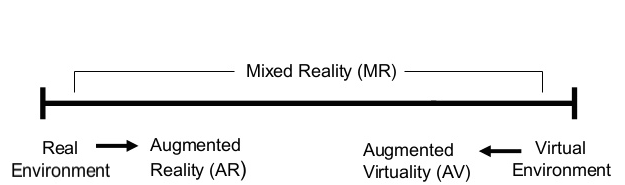
\includegraphics[scale=1]{images/ar-spectrum.png}
\caption{A spectrum overview of mixed reality technologies (Milgran 1994)}
\label{fig:ar-spectrum}
\end{figure}

AR has been used in a number of disciplines, ranging from medicine to entertainment to construction \cite{azuma_recent_2001}. It seems that there has been no previous research done on the possible application of AR in the fitness sector and therefore insights will be drawn from other applications of AR. Special focus will be paid to pedagogical applications of AR with the hope of drawing parallels between teaching in a classroom and instructing users to perform exercises in the gym. 

The use of AR in classrooms has been trialled by many and there is plenty of research evaluating it's effectiveness. AR in classrooms has been widely used in the past on desktop machines \cite{iordache_comparison_2009} but it's true power has only been unleashed recently, as the shrinking of technologies has allowed AR to migrate from desktop to mobile devices \cite{squire_augmented_2007}. Squire and Klopfer studied four different groups of students using an AR game in which students took on the role of environmental detectives. One of the main advantages of AR highlighted in their study was the ability to trigger the recollection of preexisting knowledge \cite{squire_augmented_2007}. "Learning is contextual" \cite{liestol_learning_2011} and so, by placing students in a familiar environment, they are more likely to recollect what they previously learnt in that same location. This is supported by the pedagogical psychologist Greeno, who put forward the theory of situativity, arguing that immersing oneself in the context of a situation aids with its understanding and recollection of previous relevant information \cite{greeno_situativity_1998}. Situativity is an extremely powerful tool and the gym application must exploit it. Ergo, using situativity should be one of the main requirements of the application. By simply by placing users in the correct environment, they will have a higher chance of recalling and learning the correct form of an exercise. All in all, the advantage of situativity as well as the evidence that suggests AR is an effective way to visualise information and instructions \cite{squire_augmented_2007} suggest it is a suitable technology for instruction should therefore be used in the gym application.

\textbf{Requirement I:} \textit{"Exploit situativity through location based interaction"} \label{requirement_I}


Iulian Radu expanded on the initial research of using of AR in classrooms. Similarly to Squire and Klopfer, Radu noticed a number of specific positive impacts that AR can have on learning. In Radu's experiment, AR increased understanding and the long-term retention of taught content as well as the student's motivation\cite{radu_why_2012}. Unfortunately, Radu also noticed some usability difficulties and fluctuating levels of understanding between students \cite{radu_why_2012}, hinting at the fact that design and usability are key in AR applications. Others, such as Liestøl, have realized the possible difficulties in adopting AR in the classroom but Liestøl stated that "the threshold for entering this technology is not insurmountable - it is actually relatively easy"\cite{liestol_learning_2011}. Indeed, the benefits that AR brings, such as improved learning, higher retention and motivation are extremely positive but they do come at a cost. The initial adoption of AR may bring with it some issues but if resolved, the prospects of AR are truly impressive. In  pedagogy, most teachers would need to create their own AR applications, or use ones that are specifically targeted at their syllabus and at what they are trying to teach students. This does not apply in the context of the gym app since there is no need for each individual user to re-create the app because the exercises they are trying to learn are not unique to them. This removes a significant barrier to the use of AR in the gym and all that is left to do is for the user to familiarize themselves with the AR app - just as they would with any other non-AR mobile application. 
%TODO argue the last point better
\textbf{Requirement II:} \textit{"Ensure the application is usable in any environment and with any brand of equipment"}  \label{requirement_II}

Yet another advantage of mobile AR applications is that they allow the users to move around the scene and explore different angles and perspectives of the rendered object, thus catering to a more dynamic and interactive learning experience\cite{fitzgerald_augmented_2013}\cite{dede_immersive_2009}. Kerawalla et al. carried out an experiment where AR was assessed against other, more traditional, methods of teaching a class \cite{kerawalla_making_2006}. In total, 133 children grouped in different classes attended the experiment. Each class was split into three groups and each group was then run through two sessions about the solar system using different teaching methods. There were four variations to the teaching styles: Teaching using AR by a teacher who is an expert in AR, teaching using AR by a teacher who had no prior experience with AR, teaching using the classic lecture and bookwork combination and finally teaching using the BBC ReviseWise website where kids work mostly independently at the computer. The debate during class was analysed and the teachers were interviewed after the class. One of the main outcomes of the experiment was that teachers saw the value in AR making "traditionally inaccessible subject matter available to the children"\cite{kerawalla_making_2006} and thus enriching their learning experience. In the study, the inaccessible subject was the solar system but in the context of the app, AR will be used to substitute a fitness instructor. Kerawalla et al. did not go as far as to assess the amount of information kids learned during the AR session in comparison to the sessions taught in more traditional styles but one teacher highlighted that thanks to using AR, a student "can see that picture in his head rather than just being told it, or like with a globe and a torch representation ... having to work out what stands for what"\cite{kerawalla_making_2006}. All in all, the teachers found that AR made "the  subject  matter  accessible  and real". Using AR to demonstrate how things work and replacing old, mundane methods seemed to be very effective and is also one of the requirements of the gym application.  

\textbf{Requirement III:} \textit{"Eliminate the need for an instructor to demonstrate an exercise"}  \label{requirement_III}

One of the main issues with AR technology in general is alignment with real world objects \cite{sood_pro_2012}. Object recognition, especially on mobile devices, does not yet have the needed fidelity to be able to distinguish the same object in different variations. For example, object recognition could be used to recognize a bench in the gym, however, it will only be able to recognize that specific type of bench. In a different gym, with different benches or even with the same bench but different lighting, shadows and perhaps colour, object recognition will do us no good. One possible solution, proposed by Rekimoto and Ayatsuka is to have visual tags on the objects and use these to identify them \cite{rekimoto_cybercode:_2000}. Objects that fall in the same category can be grouped together simply by being given the save tag and placing it in the correct area. Image recognition is then used to recognize the tag which servers as an anchor for the augmented reality overlay. This solves the issue of alignment because there is no need to know where the object that we are projecting the visualization onto starts and ends, instead the size and orientation of the marker is simply used to draw the visualization. Then, by constantly tracking the position, orientation and size of the visual tag, the augmentation is moved and re-sized accordingly.

\textbf{Requirement IV:} \textit{"Ensure that there are no issues with alignment or target recognition"}  \label{requirement_IV}

Having a virtually augmented layer in the users view provides a new interface for human computer interaction, but to what extend is this virtual interface effective? Balog et al. used AR glasses and a 'paddle' to point at and select virtual objects as a part of a class room exercise. Their research identified a number of issues with this interface method, most important were the inability to select every element due to overlapping objects, poor maneuverability, the paddle blocking the view of the user and a lack of tactile feedback \cite{balog_augmented_2007}. Despite these shortcomings, a group of 32 students scored the AR exercise as exciting (4.16 on a 5 point scale) and gave scores of 4.38 and 4.34 respectively for understanding of the lesson and readability of the presented information\cite{looser_evaluation_2007}. On the other hand, interacting with the virtual objects using the 'paddle' was ranked lower, at only 3.06 out of 5\cite{balog_augmented_2007}. Looser et al. also experimented with different input methods, testing selection with a virtual hand and two methods which used virtual pointers\cite{looser_evaluation_2007}. Both uses of pointers performed poorly, with error rates falling around 45\%\cite{looser_evaluation_2007}. The virtual hand performed much better but still suffered from a 20\% miss rate\cite{looser_evaluation_2007}. These findings suggest that, especially for smalls screen mobile devices, it is better to choose  more traditional methods of user interaction instead of opting for a virtual interface. Based on this, the gym application will implement a touch screen interface, with standard on-screen buttons rather than using a fully augmented virtual interface. 

\textbf{Requirement V:} \textit{"Create an easy to use on-screen graphical user interface"}   \label{requirement_V}


Perhaps the most important issue when creating a phone app in general and an AR app in particular, is the issue of attention tunneling \cite{radu_why_2012} \cite{biocca_attention_2007}. Attention tunnels, such as oncreen indicator that point the user in the correct direction to point their phone have previously been used with impressive success\cite{biocca_attention_2007}. In one experiment, attention funnels increased "the consistency of the user’s search by 65\%,  increased search speed by 22\%, and decreased mental workload by 18\%" \cite{biocca_attention_2007}. Clearly, attention funnels can extremely useful but since using AR is a relatively immersive experience, we must take care to draw the users attention to the appropriate stimuli and objects in order for them to not completely loose track of their environment - especially in the gym, which could be potentially dangerous. Biocca et al. have pointed out issues with attention funneling in mobile interfaces, stating that "the attention demands of current interfaces such as cellular phones and PDAs may play a significant role in automobile accidents" \cite{biocca_attention_2006}. Some AR applications such as \textit{Pokemon Go} have solved the issue of attention tunneling through pop ups that remind the user to stay aware of their surroundings \cite{hollister_drivers_2016}. A similar approach should be adopted in our application to ensure the users safety and must be one of the high priority requirements. Fully immersive virtual reality has been found to have positive effects on the transfer of knowledge from theory into practice in the real world\cite{dede_immersive_2009}, making immersion an important feature however "lesser degrees of immersion can still provide situated learning" and all the benefits that come with it\cite{dede_immersive_2009} and therefore by limiting immersion there is no trade off in situativity or effectiveness of information delivery.

\textbf{Requirement VII:} \textit{"Avoid users from becoming fully immersed into the application"}  \label{requirement_VI}


\subsection{Meeting with GUSA}
When developing an app of any kind it is important to consider how it is going to be marketed and distributed once finished. This question is particularly interesting for this app since it requires real-life components such as gym equipment and  markers to work. The app also finds itself in the midst of a two sided market place, needing to be sold to both gym owners and gym goers. As a result, both the gym owners and gym goers must be considered as customers and consulted during the creation of the app. As a result of this, before research and development even begun, a meeting was arranged with the president of the Glasgow University Sports Association (GUSA) and the Sport Development Manager at Glasgow University Gym. The meeting was held on the 26th of July 2016 and yielded a number of interesting requirements and points of discussion, many of which had not been previously considered. 

One point of discussion was the issue of liability. The main goal of the app is to demonstrate what perfect form of an exercise looks like, however there are conflicting views as to what 'perfect' form for an exercise is and how to execute it. Most of the times there will be a theoretical ideal motor pattern to lift the most weight efficiently, however when a user tries to recreate this, they might be put in a compromising position. Take, for example, the deadlift (picking up a bar from the floor and finishing in a standing position with the bar mid thigh). Within the app, it may be demonstrated that the safest starting position is from a half-squat where the thighs make a 25° angle with the floor. This may indeed be the safest position for someone with a perfectly proportionate body, but if somebody has shorter arms and longer legs, they may need to squad down further to reach the bar and be in a strong position. If such a user were to follow our instructions too closely they may round their back in order to reach down to the bar and end up hurting themselves. If a user was so inclined, they could blame the app for providing unsafe instructions to them. A potential solution would be to show a disclaimer within the app or during app launch that notifies the user that all demonstrations of form are approximate and that the user should contact an expert if they are unsure how to properly and safely perform an exercise. If a user is clearly made aware that the demonstrated form for each exercise is only approximate and shows what the creators deemed most efficient, then there should be no liability issues. 

\textbf{Requirement VII:} \textit{"Show theoretically perfect form and notify user of any dangers"} \label{requirement_VII}

GUSA was cautious about how the app is going to be distributed and marketed since they are themselves working on a designated GUSA app and are also pushing the LifeFitness app to their customers. The main concern was that by having too many apps marketed in the university gym, customers would be overwhelmed and end up using none of the apps. It was decided that in order to solve this dilemma, the app will be tested in the Glasgow University Gym however will not be distributed by GUSA nor will it have any relation to GUSA. 

\section{Acceptance Criteria}
Having review the appropriate literature and elicited requirements from GUSA, it is good practice to now also determine how the success of these requirements will be monitored. What follows is an outline of acceptance criteria for the different requirements. These criteria will be refereed to throughout the project to track progress and at the conclusion of the project to evaluate the end product. 


\begin{table}[]
\centering
\resizebox{\textwidth}{!}{%
\begin{tabular}{p{2cm}p{5cm}p{5cm}p{5cm}}
\textbf{Requirement Number} & \textbf{Requirement Text} & \textbf{Guiding Question} & \textbf{Acceptance Criteria} \\ \hline
I & Exploit situativity through location based interaction & Is the app usable in the gym? Is there utility from using the app in the gym as opposed to at home? & User feedback \\\hline
II & Ensure the application is usable in any environment and with any brand of equipment & Does the app work anywhere and with any brand of equipment? & Test app with multiple manufactures/in multiple environment \\\hline
III & Eliminate the need for an instructor to demonstrate an exercise & Can users use the app and gain knowledge by themselves? & User feedback \\\hline
IV & Ensure that there are no issues with alignment or target recognition & Does the tracking work well? & User feedback \\\hline
V & Create an easy to use on-screen graphical user interface & Do users understand how to use the app? & User feedback \\\hline
VI & Avoid users from becoming fully immersed into the application & Is there any way to avoid users getting sucked into the app? & Observe users as they use the app \\\hline
VII & Show theoretically perfect form and notify user of any dangers & Are users aware of any possible dangers? & User feedback \\\hline
\end{tabular}%
}
\caption{An overview of acceptance criteria for the project}
\label{acceptance_criteria}
\end{table}

As can be seen in table \ref{acceptance_criteria}, the success of a number of the acceptance criteria will be determined by collecting user feedback, which will be done by running user trials on a number of occasions. For the purpose of this project, user testing is more suitable than automated testing since user testing provides much more substantive feedback. Furthermore, since the app will not be taking in any input from the user and works in a \textit{closed circuit}, having automated testing wouldn't bring much benefit as there are no viable input to trial. The app will be developed in multiple iterations, each concluded by customer meetings or user testing in order to monitor progress and gain insights into what the user expects.  When running user tests, a representative sample made up of both male and female individuals who have mixed experience in the gym must be used. Other demographic indicators such as age, experience with technology etc. may also be important however since testing is to be performed at the university, it may be difficult to assemble a well distributed sample group. Despite this, since young adults are the target audience of the app anyway, the user testing should yield interesting and objective insights into what the consumer expects from the app and how it can be improved. 

% \chapter{Design}
% \section{User Interface}
% The quick brown fox jumped over the lazy dog.
% The quick brown fox jumped over the lazy dog.
% The quick brown fox jumped over the lazy dog.
% The quick brown fox jumped over the lazy dog.

\chapter{Implementation}
The development of an augment reality phone application sounds quite daunting at first. The image recognition, 3D object mapping, use of sensors and mathematical calculations to pivot the projected image are undoubtedly complex however, there are many libraries and tools that allow for the abstraction of the complicated and intricate work, drastically simplifying the development of the core of the app. Despite this, the initial learning curve to find, set up and get started with all the tools and technologies is very steep. In order to make the process easier implementation will be broken down into three iterations which will build upon each other incrementally and allow for frequent feedback. In this section we are first going to explore the numerous tools used throughout the project, justify their selection and talk about how they are used. Later each of the three iterations will be examined and some of the major events, decisions and problems will be highlighted.

\section{Technologies used}
\subsubsection{Git}
One of the first tools that was set up as a part of the project was the Git version control system. Git is usually used in the open source community or within teams to allow easy integration between contributors. For the purpose of this project, Git is used to keep a backup of old versions of the app and to share the progress of the project with the project supervisor. There are many other version control systems such as SVN or Merculiar. Git was chosen due to my familiarity with it and due to the fact that it is a de facto industry standard.
	
\subsubsection{Vuforia}
Vuforia is one of the many open source augmented reality libraries \cite{vuforia_getting_2016}. Vurofia was chosen due to it's simple integration with the Unity game engine and it's well documented Android code development SDK \cite{rao_how_2015}.. Vuforia provides an online interface where users can upload different images which are then analysed for specific feature patterns that are used for matching. For example, figure \ref{fig:coca_cola_features} show the feature patterns of a CocaCola logo. A collection of such targets can be exported as a database and later used in Unity for matching using optical recognition \cite{rao_how_2015}.
\begin{figure}
\centering

\includegraphics[scale=1]{images/coca_cola_features.png}
\caption{Patterns of features on the CocaCola logo.}
\label{fig:coca_cola_features}
\end{figure}

\subsubsection{Unity}
Unity is a well known 3D cross-platform games engine that is widely used in the field. There are many other game engine alternatives, however, Unity was chosen due to it's seamless integration with Vuforia and MakeHuman. Unity also allows us to export into different platform native application and so, even though Android is out target development platform it would be relatively easy to port the application over to an iOS device or Windows mobile. 

\subsubsection{MakeHuman}
MakeHuman is a humanoid modeling software that makes creating life-like humanoid figures very easy. MakeHuman has a simple interface which allows the users to customize and configure their character. Many open-source on-line forums are also dedicated to creating a large database of download-able body parts and clothing, enriching the variety of customization that MakeHuman provides.

\section{First Iteration}
The goal of the first iteration was to create an initial functioning prototype that would serve as a proof of concept regarding the use different technologies and explore how best to achieve the desired objectives. 

\subsubsection{Logical Layout}
One of the first major issues encountered was concerning the logical layout of the application. The initial intention was to create the core AR functionality of the app in Unity and then export the project into Android Studio where the other views such as the home screen, setting page etc. would be created. It took a couple days to set up the development environment, learn about app development for Android and to complete the starting tutorials. The next step was to export the Unity project into Android Studio and build a home screen that would load on start up and allow the user to navigate to a camera view which would contain the AR part of the app. Unfortunately, whenever the user would switch between the two views, the Unity launch screen would show up. This is undesirable for two reasons. First, showing the launch screen slows down the use of the app as it introduces unnecessary latency. Secondly, showing a splash screen in-between two of the main views deteriorates the natural flow within the app since splash screen are usually shown on start up and could cause users to get confused about how to navigate between views. Furthermore, showing a seemingly random branded splash screen in the middle of the app takes away from the brand and united design that the app should have. 

A number of fixed were trialled in order to remedy this issue. One attempted solution was loading the camera view first on start up and then automatically switching to the home view once the splash screen loaded. While this did successfully show the splash screen on launch, it did not solve the problem because the splash screen would still show when switching onto the camera view. Modifying the automatically generated unity files to stop the splash screen showing up all together was also considered but research has shown that this would violate the Unity terms and conditions. In order to remove the splash screen legally, a full professional version of Unity would have to be purchased (TODO: Cite unity) which is not an option due to financial constraints of the project.

The solution arose organically as a result of increasing familiarity with the Unity development environment. While building the user interface for the Augmented Reality camera view, an inbuilt tool for creating interfaces within Unity was discovered. This tool makes it possible to create all of the graphic interfaces needed for the app within Unity. Then, by attaching scripts to different components, the menu can be made more dynamic and allow for the implementation of more advanced functionality. Other features and views can be created in separate scenes which can be routed between. The main disadvantages with this approach is that all development will need to be carried out within the Unity editor, granting less fidelity than native Android development. Furthermore, an unfamiliar language, C\#, will have to be used as opposed to Java.

\subsubsection{Animations}
Animations play an important part in the app and are highly representative of it's design. Due to the specificity of the movements needed for the app, only a handful of exercises were found on-line in open-source repositories. For the purpose of this project a full suite of exercise animations is not necessarily required however in order to provide a realistic representation of how the app would look when complete and to validate the development process, at least some custom exercises must be created. After investigation it was decided that Blender is the most suitable tool to use to create the animation because it provides a detailed and complex interface for professional animation and is compatible with Unity. The two main issues with creating animations have been a lack of experience with animating and with Blender, deeming the complex graphical interface of Blender to be quite overwhelming at first. The learning curve was made worse by the fact that some of the key-bindings were, by default, overlapped because development was carried out using a laptop which did not have a full numerical pad unlike a desktop PC with a designated keyboard. Thus whenever a key was pressed to switch view using the top row numbers, different bones would get copied making the animation jump back and forth when run. This was because the top row of keys was assigned to copying different bones and also assigned to switching views. Reassigning the key bindings solved the issues however it took a long time to identify what was going on and the learning curve for all the other features was still significant.

Even after learning how to use Blender and how to animate, it was still difficult to know exactly what form exercises should have. In order to present an accurate and safe representation of each exercise a reliable point of reference was necessary. Rather than combining different sources and compromising on form, it was decided that picking a single reputable source and basing all animations on it was the best solution.  The exercise database on bodybuilding.com provides a varied range of exercises with plenty of description both in text and images making it a suitable choice. Even with a clear intention and method on how the animation should look and how they are made, the actual creation of the animations is extremely time consuming, meaning that the total the number of animations that are going to be self-created must be limited.

\subsection{2nd Meeting with GUSA}
At the end of the iteration, a second meeting with the president of GUSA took place in order to discuss progress on the application and gather feedback from an expert in the field. During the meeting, which took place on the 15th of November 2016, the application was demoed and the president was asked for his opinion on a number of design choices and possible features. At the time of the meeting the application was largely at a proof of concept stage. Consequently, the design of the application (as can be seen in figure \ref{fig:it1}) was temporary and much of the discussion during the meeting revolved around possible additional features that could be implemented in the future. 

\begin{figure}[h]
\centering
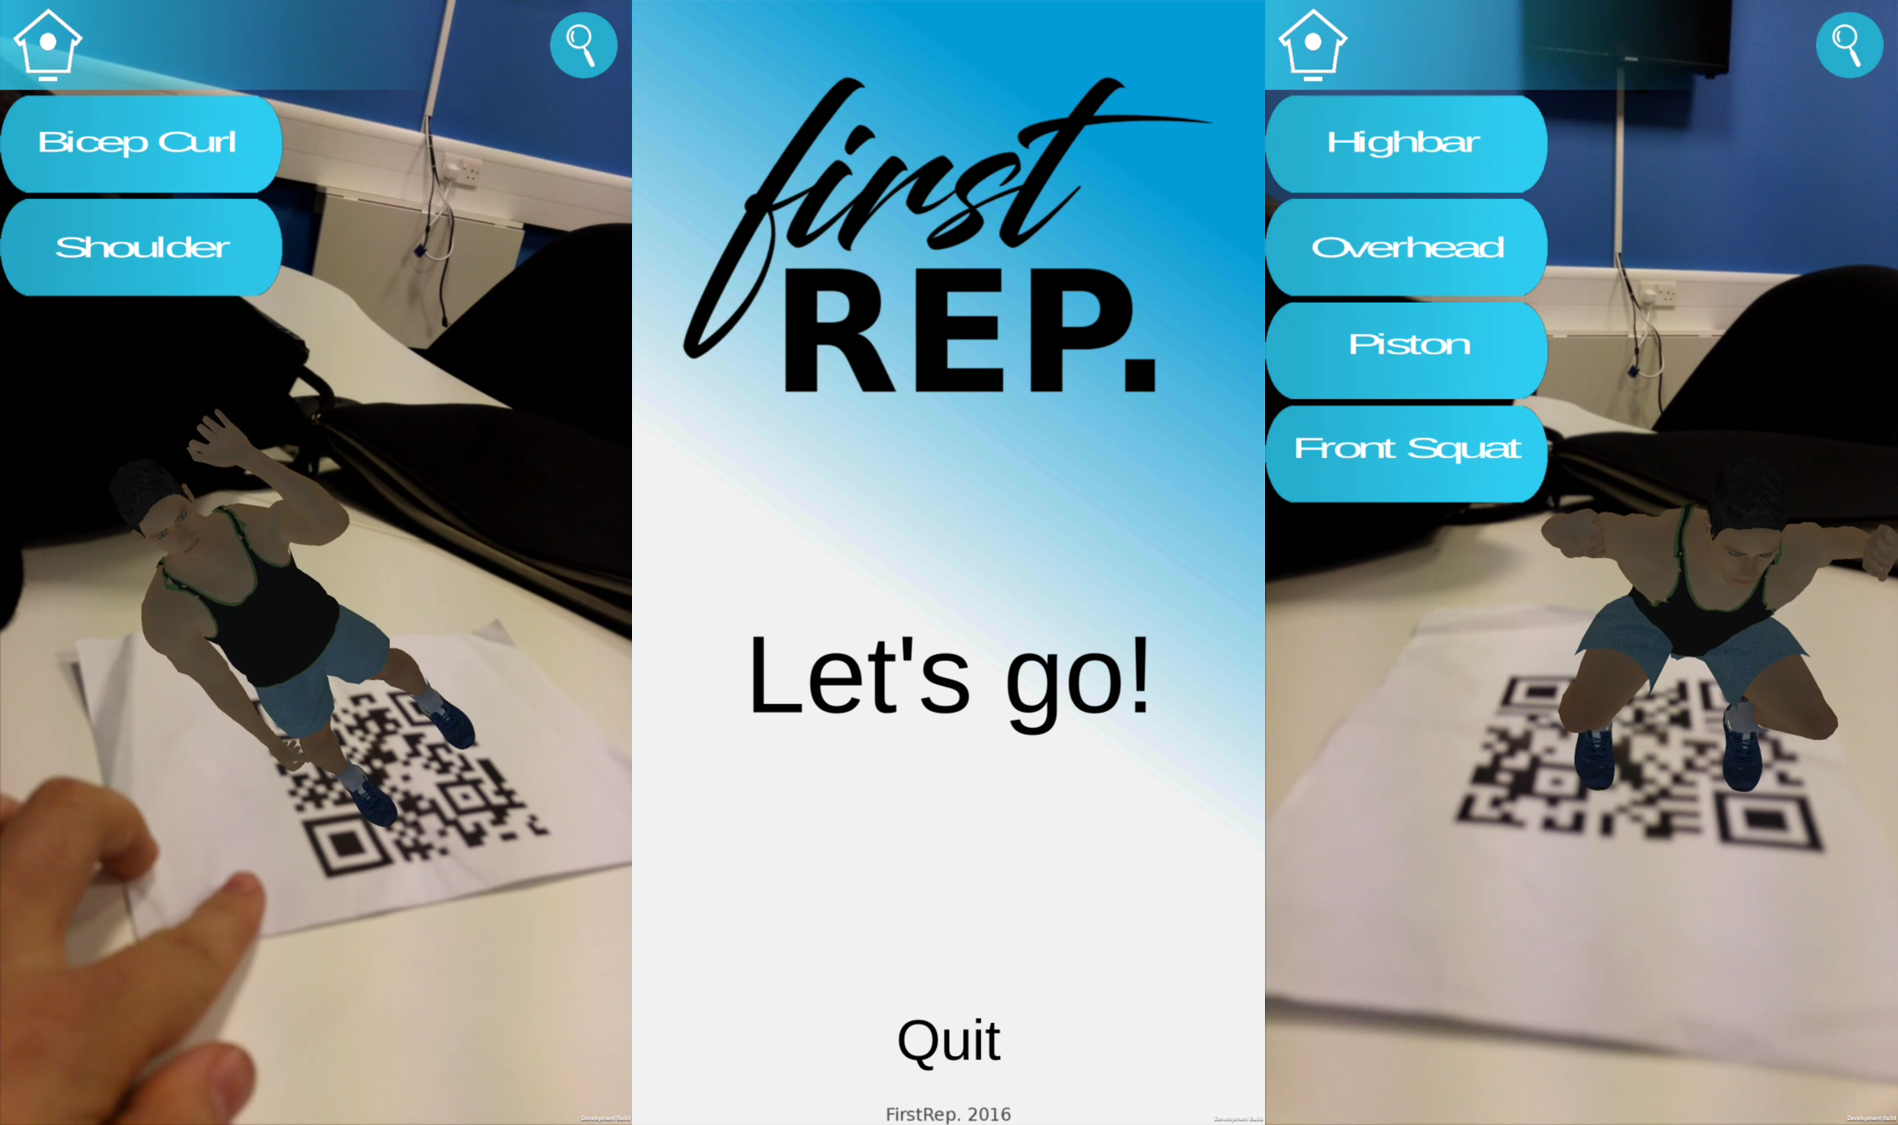
\includegraphics[width=\textwidth]{images/iteration1_screenshots.png}
\caption{Screenshots to show the state of the app at the end of the first iteration}
\label{fig:it1}
\end{figure}

Perhaps the most important outcome of the meeting wit GUSA was a reminder to the agreed upon size of the QR codes. In the initial meeting it was decided that the QR codes should be about the size of a postage stamp in order for them to blend into the equipment and cause as little distraction as possible. However, until this meeting, only large QR codes that took up about half a page of A4 paper were used during development, simply because that is how they came out when first printed. So far, the size of the QR codes was completely ignored, under the assumption that it would be trivial to shrink the QR code down when need and simply change the ration of the augmented character to the marker, however this was not the case. By shrinking the QR code and tweaking the ration to make the avatar human size, the user is forced to step back away from the marker when using the app in order to fit the entire avatar into the screen view. It can be quite awkward for a user to have to come close to a machine, scan the QR code and then take a step back, all while pointing the phone in the correct direction. Furthermore, if the avatar appears right when the user scans the QR code, the user will be way too close and their entire screen will be filled by just one body part of the avatar. It might be the case that we will have to calculate the distance between the user and the QR code and perhaps tell the user to step back until they are far enough to see the entire avatar - this could be potentially tricky and needs to be explored in the next phase of implementation. 

Overall, the GUSA president was quite impressed by app so far but was also aware of the fact that much more work is yet to be done. The meeting helped justify and confirm many of the design choices that were made. Furthermore, new features were also suggested and explored. For example, the president thought it would be useful to have a browse feature where exercises can be views in groups sorted either by either equipment or target muscle group. When the user would select an exercise in the browse view, it will be rendered on the screen just like if the user triggered the exercise by scanning a QR code however the character would be stationary instead of panning on the users motion. It's not clear exactly how much benefit this feature would bring to the users and so this question remains to be answered by future user trials. Another suggestions was to include equipment in the animations and haven an option to toggle it on and off in order to not obscure the users view of the exercise. It was also decided that an about page which will explain how to safely use the app should be included, alongside having pop ups with safety disclosures that remind the user to stay safe and pay attention to their surroundings at regular intervals. User testing was also discussed and agreement was reach to carry out the tests at the Glasgow University Gym at the end of the next iteration.

\section{Second Iteration}
The intention of the second iteration was to act on some of the feedback that came from the meeting with GUSA and get the app ready for user trials.

\subsubsection{Redesign}
First impressions matter and in terms of software these impressions are often made through the design of the user interface. For the purpose of the first iteration, design was not a priority, ergo a redesign was due in the second iteration. The main focus of the redesign was the home page because that is what a user sees first and most frequently. As can be seen in figure \ref{fig:it1}, the initial design only had two buttons on the main screen. Both buttons were plain text, with the top button taking the user to the AR camera and the quit button closing the application. During the redesign, it was decided to include more buttons and make them more obvious. This was both a design choice and a bi-product of the newly added info and search screens. The "quit" button was left out because Android provides a hardware key to exit from applications and there is no need to duplicate the functionality. The redesign of the home-screen can be seen bellow in Figure \ref{fig:it2_home}.

\begin{figure}[h]
\centering

\includegraphics[height=8cm]{images/redesigned_homescreen.png}
\caption{Screenshot to showcase the new design of the home screen}
\label{fig:it2_home}
\end{figure}

\subsubsection{Tracking}
The staple piece of functionality of the app is the tracking of markers and the display of animations in AR. The logic of how this functionality should work is relatively simple but it's implementations has proved to be quite challenging. The principle is to open up the camera and try to detect a marker that contains a specified pattern of features. Once a tracking has been acquired, a 3D character is displayed and an animation is played. As the user moves around the market, the character is rotated, zoomed and paned based on the movement of the phone in relation to the marker. There are libraries such as Vuforia that abstract much of the heavy lifting to do with tracking markers and moving animations on screen, however they are not perfect. The single largest issue has been the detection and tracking of targets. In the meeting with GUSA at the end of the first iteration, the size of the QR codes was deemed too large and the size of the avatar deemed too small. The process of scaling down the QR code and enlarging the character was trivial and simply involved changing the ratio of the image target and the character however the new relative sizes gave rise to a subtantial issue.

Having a small tracking target severely decreased the usability of the app because the user has to get close enough to the target for the camera to recognise it and then has to step back far enough to fit the entire figure into view. There are several problems with this. First, as the user is stepping back they are likely to move the phone around, thus moving the target out of view and loosing the tracking. Secondly, even if the user stands far back enough to see the entire figure, the target being used as an anchor is so small that recognizing it and it's exact orientation is difficult for the camera, causing flickering and misalignment. Lastly, the process simply involved too much movement which is not only inconveniently but also potentially dangerous. As a user is walking backwards and trying to keep the tracking active, they may walk into objects or people behind them, risking injury. 

It is difficult to make decision on how to fix the issues with alignment and proportions of the character and the markers without any user feedback. For this reason, the character will remain life sized for now and in the user testing, the usability of this set up will be evaluated and changes can be made in the following iteration based on the gathered user feedback. 

\subsection{User Testing}
In order to assess the degree to which the application is fulfilling the set out requirements and objectives, user testing was carried out on the 18th of December 2016. The testing took place in Studio 1 of the Glasgow University Gym and participants were brought in individually to test the app. Each attendant was briefed concerning the privacy and anonymity of any collected information. Furthermore, the participants were made aware that they may withdraw at any time or ask for their data to not be used. Each test consisted of two main parts. First the user was asked to use the app to carry out some possible user scenarios, which can be seen in Table \ref{test_scenarios}. The users were asked to speak out loud as they were thinking in order to identify any points of friction while using the app. Some trails were recorded using screen recording software for future reference.

\begin{table}[h]
\centering
\caption{User scenarios used in testing}
\label{test_scenarios}
\begin{tabular}{ll}
1 & Find out how to do the piston squat.\\
2 & What exercises can be done at the curl station? \\
3 & Find the search page \\
4 & Find the info page \\
5 & What is the last station used for (referring to the deadlift platform)
\end{tabular}
\end{table}

The second part of the trial consisted of a short anonymous survey which the participant filled out without supervision. The questions asked in the survey can be seen in Appendix \ref{survey}. Results of the survey are summarized in Table \ref{survey_results}.

\begin{landscape}
\begin{table}[ht]
\centering
\resizebox{23cm}{!}{\begin{tabular}{p{2cm}p{2cm}p{2cm}p{2cm}p{2cm}p{2cm}p{3cm}p{3cm}p{2.9cm}}
\textbf{Participant} & \textbf{Gender} & \textbf{Gym frequency} & \textbf{Design} & \textbf{Ease of use} & \textbf{Likelihood of future use} & \textbf{Best feature} & \textbf{Improvement necessary} & \textbf{Further thoughts} \\ \hline
A & M & 3 & 3 & 3 & 1 & You get to see the movements visually. & There could be text added to make it more informative. & N/a \\ \hline
B & M & 5 & 5 & 5 & 1 & Animations showing exercises & QR code allignment & Add more exercises and try to get a clearer animation view \\ \hline
C & F & 5 & 4 & 5 & 5 & Easy to use, very clear and helpful & The quality & Really good idea, would be very popular! \\ \hline
D & F & 5 & 5 & 4 & 5 & the idea in general, sometimes when you go to a new gym you dont know the new types of equipment, so this would really help & you need to learn to lean back rather than just tilting your phone, but once you understand that you need to do this it works really well & clever design \\ \hline
E & F & 1 & 3 & 5 & 4 & good use of qr & better visuals & so much potential for ad-ons \\ \hline
F & M & 4 & 5 & 5 & 5 & The full 3D animation allows you to see how to improve form accurately. & Probably keeping the animation up whilst walking around the QR code. & Would be very good for beginners as I personally would have loved to have had an app available to help me improve my form. \\ \hline
G & F & 3 & 4 & 3 & 4 & I liked being able to see the exercise from 360degrees. Makes it clear what to do :) & Stop it disapearing all the time & Would be good to see other (non-lifting) exercises - like yoga \\ \hline
H & M & 5 & 5 & 5 & 2 & Good for beginers & More exercises & Give more info on how to use the app \\ \hline
\end{tabular}}
\caption{Results from the 1st iteration of user testing}
\label{survey_results}
\end{table} 
\end{landscape}

After examining the data from the user testing, it can be see that the participants consisted of a mixture of male and female and had varying levels of experience in the gym, making our sample somewhat representative of the target audience. In the trial, the design of the app scored well, achieving a mean average of 4.25 out of 5. The users also found the app easy to use, giving it a cumulative average score of 4.375 out of 5. While these scores are encouragingly high, perhaps the most important metric - the likelihood of use, was quite low, scoring only 3.375 out of 5. What is more, the data is quite spread out and has a standard deviation of 1.77, which is significant in a scale of only 5. We can also observe a tendency for users who are frequent gym goers to be less likely to use the app (especially participants A,B \& H). This is likely due to the lack of variation in the exercises presented in the demo. These participants did not see the utility in using the app since they already knew all the exercises demonstrated in the app. This claim is echoed in the qualitative user feedback with participants D, F \& H all stating that the app is "good for beginners" (Participant H). As a remedy, and to make the app more useful, some of the participants (A,B,E,G \& H) suggested adding more exercises as the single most important improvement. Participant E identified the opportunity for having add-ons in the form of workout packs and Participant G commented that the app could be used to demonstrate yoga exercises. Contemplating this feedback has brought up the idea to provide a \textit{freemium} service where every user receives a basic set of exercises and can pay to download additional packs of exercises that are grouped together by a common theme such as yoga, Olympic weightlifting or stretching. 

Coming back to the user data in Table \ref{survey_results}, it is clear that the design of the application was generally received well but some issues were identified in the qualitative feedback. All participants, except H, commented on the poor usability, alignment or quality of animations in the app. During use, many users struggled to keep the animation tracking because as they moved around, they would loose the QR code from the view-port and the character would disappear. This is clearly an area for future improvement. As Participant D pointed out, "you need to learn to lean back rather than just tilting your phone, but once you understand that you need to do this it works really well". Therefore a possible solution would be to include a prompt which shows up when the user first uses the app and instruct them how to track with the phone in such a way that the animation is not lost. This approach could yield some improvement however perhaps a better option would be to configure the tracking to not disappear if the marker is lost in the y-axis. Thus, if the user pans up and down with the device, the animation stays rather than disappears due to the marker being bellow the field of view. 

One of the key questions that was to be answered during this iteration was how, if at all, to implement the browse functionality put forward by the GUSA president. Making information about how to perform exercises easily available within the app is the principal objective however having both a reactive augmented reality view and a static view may be confusing to the users. The development of the browse  function was therefore halted and instead only a quick prototype version of this feature was created. During the testing, users were asked if and how they would use the browse function. The majority of users thought the browse function was a good idea and were able to navigate to it in the app and understand it's purpose. The users were asked as to what they expect to happen when they click on an exercise in the browse view and almost all users wanted to see the animation of the exercise appear on screen (even though there is no marker). This animation would not track along with the sideways movement of the phone and instead be stationary, allowing the user to look at exercises in any setting. Thanks to the positive feedback about this feature, it will be implemented in the next iteration.

\section{Third Iteration}

\subsubsection{Search}
Given the positive feedback gathered in the user testing about the search function it was decided that this should be the main focus of the third and final iteration. Ideally the view would be searchable and have a reducible list that would narrow down the search result as the user typed however due to time constraints it was decided to instead provide the user with two separate browse views - one which is grouped by the trained muscles and the other by equipment used. Having a scrollable list that is dynamically generated and has two view options posed a number of technical challenges. Initially the idea was to have a default template view where there would be one category element with one child element. Assuming the default view was the muscle view, each of the category elements would be cloned for each of the muscles. Then, for each muscle, the exercises would be added by cloning the child of each of the category elements. When the user wanted to switch to the equipment view, the list would be reset to the template state and the same algorithm would be run again, only this time generating the equipment list instead of the muscle list. Even though the algorithm works well in theory, in practice there is one fundamental issue. Resetting the template takes too long and so when the next population call is made, the template is still not instantiated. The reason for this is that the buttons are of type "RawImage" which is rendered at the end of the frame and the population call is triggered before that. One possible solution would be to call the reset method and then wait until the next frame to call the population method. This is quite complex and a more simple solution would be to simply have two separate the two views into separate scenes and have the application switch between them. Initially there was a concern about performance and lag however in the end switching between the two scenes ended up being quite fast and not noticeable to the user and therefore this was chosen as the desirable option.

\subsubsection{Markers}
\begin{figure}
\centering
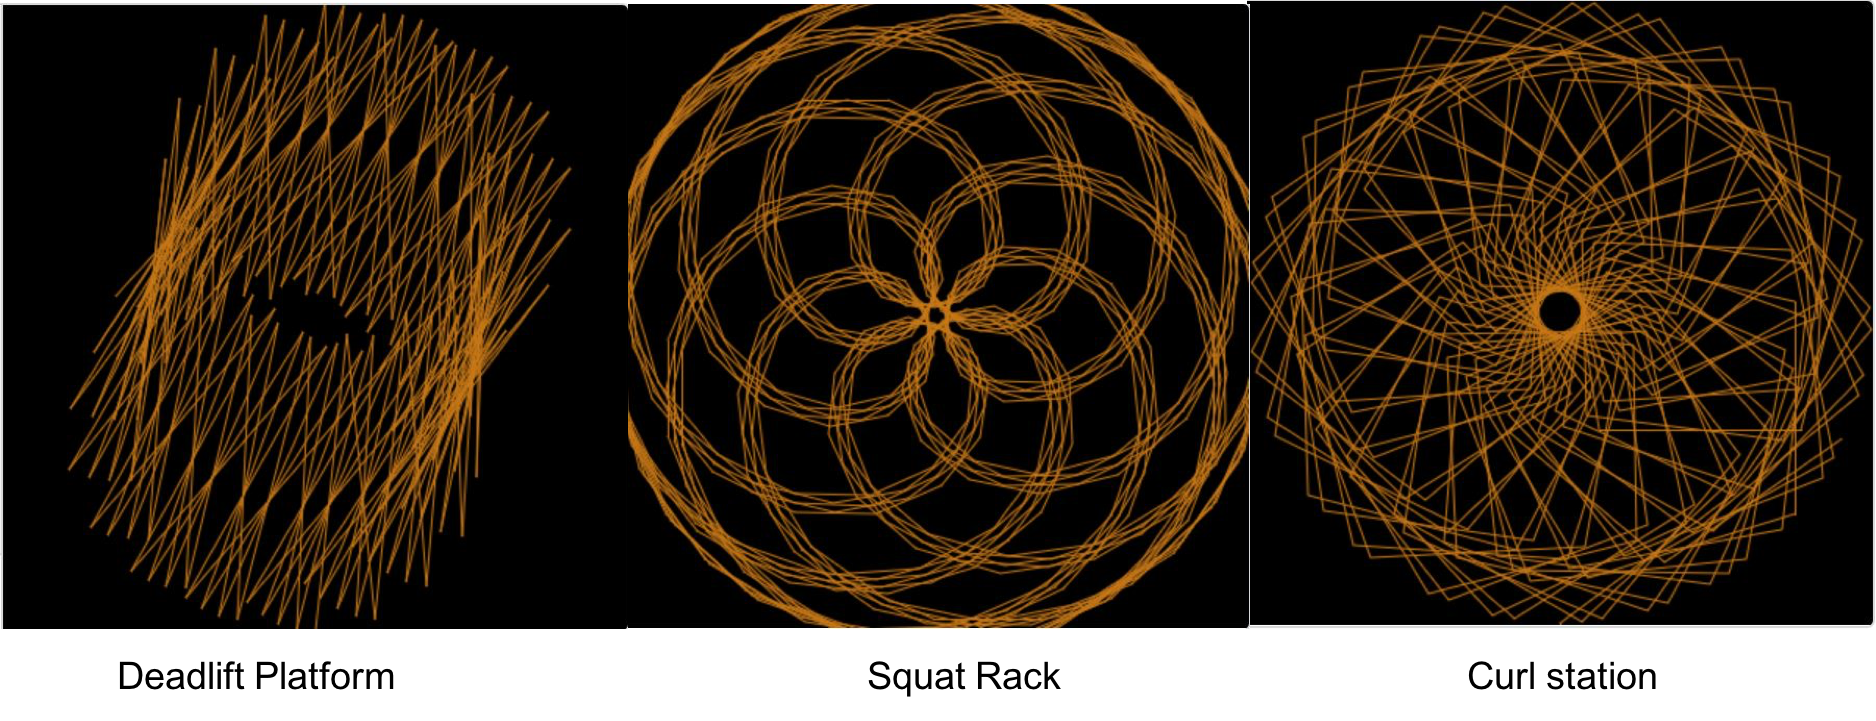
\includegraphics[width=\textwidth]{images/fractal_marker.png}
\caption{A feature rich version of the markers created using fractals} 
\label{fig:fractal_marker}
\end{figure}

\begin{figure}
\centering

\includegraphics[width=\textwidth]{images/paint_marker.png}
\caption{A version of markers that have more unique feature pattern shapes in them} 
\label{fig:paint_marker}
\end{figure}

Most of the negative feedback from the previous user trials revolved around usability of the AR functionality. Users found that sometimes, when moving around the room, the app would loose the tracking or misalign the character with the marker. Since the augmented character is life-sized the user must move quite far away from the marker in order to see the entire character on their phone screen. As the user moves away, the marker is smaller and smaller on the screen, until the marker is too small to be recognised and the tracking is lost. Initially it was though that the cause of the issue was that the QR codes used as markers were either too similar to each other to be properly distinguished or simply did not have enough features to base a tracking on. In order to test whether this was the case, a number of other markers were devised with distinct feature patterns. Three versions of this can be see in Figures \ref{fig:fractal_marker}, \ref{fig:paint_marker}. Each of the variations was tested and compared to the standard QR codes but no improvement in tracking could be seen. In fact the markers in Figure \ref{fig:fractal_marker} yielded worse performance than the original QR codes. As a result of this, it was concluded that there is a threshold, proportional to the size of the QR code and distance away from it, bellow which the tracking is lost. 

After dispelling the notion that the issue lay in the number of features that the makers had it was clear that the issue was with the process of tracking and not with the markers. One possible solution would have been to use the marker to trigger the virtual animation but then keep showing the animation after the tracking is lost. While this option would maintain the tracking, it would only work if the user was perfectly stationary. If the user would move around the animation would quickly become misaligned as there would be no anchor point to rotate the character around. This solution could be further extended to only hide the animation if the tracking was lost in the x-axis. This means that the user could pan up and down and walk close and far from the marker are not loose the tracking. When the user would turn away from the marker, the tracking would then be lost since this is the expected behaviour. While this solution works in theory it is extremely difficult to implement and the Vuforia library does not provide these option, not is there a way to access any indicative variables from the code. This solution is therefore too complex for the project and a more straight forward solution would be preferred. 

The original intention was to have the markers as small as possible for cosmetic reasons however, as described, this means that the threshold for how far away the user can be is small. An option would be to scale down the character, which would make it  easier to fit on the screen and allow the user to stay closer to the QR code, ergo not loosing the tracking as easily. However, scaling down the character bellow life-size makes the animation less realistic, which is one of the key features of the app. The alternative is to enlarge the markers. It may at first not seem favourable to do this since they will take up more space and be move obvious in the gym however having large QR codes plastered around the gym may attract more users as they will be interested in what the purpose of the QR codes is. To facilitate this marketing opportunity, the QR codes could be made into hotlinks that would open the Play Store where the user would have the option to download the app. There are no other real trade off with this option and since the tracking clearly works better with large markers, this is the chosen solution.

\subsection{2nd User Testing}
The second round of user testing took place again at the Glasgow University Gym on the 18th of February 2017. Nine users participated in the trail in total. The cohort was made up of 5 females and 4 males and had a good distribution of gym visit frequency. The test subjects were asked to execute the same user stories as in the first user trial and were asked similar questions. The participants were encouraged to speak their mind as they used the app to help identify points of friction and any possible confusion. The screen and audio was recorded while the trials were in progress in order to add context to what the user was saying while using the app. Summarized results of the survey at the end of the trials can be seen in Table \ref{tbl:2ndtest} and the full set of questions is located in Appendix \ref{survey2}. As can be seen, the 2nd survey implemented a more qualitative approach since it provides richer data for small samples in comparison with quantitative data extraction methods. Consent forms for the user trials are located in Appendix ??? along with the introduction and debriefings scripts in Appendices ??? and ??? respectively. 


\begin{landscape}
\begin{table}[ht]
\small
\centering
\resizebox{25cm}{!}{\begin{tabular}{p{0.5cm}p{1cm}p{2cm}p{3cm}p{3cm}p{3cm}p{3cm}p{3cm}p{3cm}p{2cm}}
\textbf{User} & \textbf{Gym visits (/week)} & \textbf{Design} & \textbf{Ease of Navigation} & \textbf{Ease of use (AR view)} & \textbf{Ability to learn based on animation} & \textbf{Improvements} & \textbf{Future features} & \textbf{Best feature} & \textbf{Recommend the app to a friend?} \\ \hline
A & 0 & Good overall, could improve the muscles section & Very easy & Easy but with technical issues & Yes & Improve the design of search section, improve the QR scan. & More exercises & AR View & Yes \\
B & 4 & Graphics of exercises quite good, some text is a bit blurry & Very easy & Character too big, difficult to keep QR code in view & Learn, given previous understanding & Improve menu, shrink character, add equipment & Include both genders,  option to see instructions to exercises & Very creative, useful and applicable & Probably, after improvements \\
C & 6 & Very professional, needs polishing & Easy but more features could become harder to find for a new user. back button should point left not up & quite difficult to keep the avatar on screen & link to the info screen from avatar with more detailed instructions and text & n/a & customise avatar, more detailed instructions in info with muscle heat maps & the augmented avatar & 100\% \\
D & 4 & I liked the colours, it was clean looking and nicely simple. & very easy to navigate, one hesitation point was getting back to being able to scan when i searched for a muscle group. & medium, several times I stepped too far back so lost the avatar. & Yes & Be able to change the size of the avatar to fit it to the screen better & How many times you've used/work out each muscle group to give a sense of progress & avatar showing full movements , have found it hard to have the right form by following 2D graphics & Yes \\
E & 5 & I like it, it's simple to find your way around & Quite easy, except "hide bro"" doesn't really translate to ""go back" & It was ok, sometimes the man disappeared, hard to scan the QR code & Yes & Alignment of the man with the code, he disappeared often & Nutrition tips & You can search for things without scanning & Yes \\
F & 5 & aesthetically pleasing & easy, clear what to do & the man made it clear what to do, some problem with him disappearing when QR code lost & yes & try improve QR code alignment & a women or man option for the augmented reality & scanning the QR codes to show exercises & yes \\
G & 3 & Intuitive and easy & No problem at all & Sometimes it was difficult to scan initially & Yes easily & A link to the machine name from the video of the bro & A link to the machine name from the video of the bro & The virtual bro & yes \\
H & 0 & good & easy & medium & yes & make the guy a lot smaller as you often can't see him &  & ar & yes \\
I & 0 & Functional but quite spartan & Pretty easy & Pretty easy & Yes for most of the animations & Some animations don't look quite right - I'd change those & Animations which also contain weights / machines / whatchamacallit & the VR view & yes
\end{tabular}}
\caption{Summarized results of the 2nd user testing}
\label{tbl:2ndtest}
\end{table}
\end{landscape}


%this can be moved before the graph if need be
Sourcing from the feedback in Table \ref{tbl:2ndtest}, it is obvious that the app was well received, though there are also a number of improvements that must be made to take the app from a prototype into a feasible product. All of the participants replied positively when asked if they would be willing to recommend the app to a friend, especially if some improvements were made. Furthermore, 7 out of 9 of the users thought the AR view was the best feature and despite having some issues with usability, most stated that they would be able to learn new exercises based on seeing the animations. These are important metrics since they have a significant influence on the likely hood of the app spreading and being widely used.

%Height matters
%Taller people have better perspective
%Shrinking the guy
%People were comfortable with this
%Surprising
The user testing generated a number of valuable insights. One of the most interesting outcomes of the trials was a noticeable correlation between physical height of the user and ease of use of the AR section of the app. The suboptimal maneuverability of the AR view has been discussed previously in this report but the adverse effects were experienced noticeably less by users who were taller and thus viewing the animation from a higher vantage point. Only two of the users were significantly taller than average (6'5 and 6'4) and it is therefore difficult to generalise this observation on their experience alone but it seems to be logical. Since tall users have longer arms, they are able to stand further away from the marker while scanning it and then simply retract their arms to view most of the character. Shorter users, on the other hand, have to take steps backwards in order to fit the character onto the display, ergo lowering their viewing angle. Furthermore, by having the phone positioned lower, the shorter users start with a more acute viewing angle, allowing the marker to disappear quicker \textit{beyond the horizon} (reaching the threshold viewing angle, beyond which the marker is not recognised). Combining these two set backs, as shorter users step away from the marker, the character becomes misaligned or disappears all together. For tall users, the initial viewing angle is better and less steps are needed to fit the character into view, amounting to better usability of the AR section. A graphical representation of the phenomenon can be seen in Figure \ref{fig:heightAR}. 

\begin{figure}
\centering
\includegraphics[width=\textwidth]{images/tallpeople.png}
\caption{Diagram of how user's height effects usability of the AR functionality} 
\label{fig:heightAR}
\end{figure}

Enlarging markers helps with tracking over longer distances, however viewing angles are still a problem, especially near the threshold values. When the 2nd user who completed the user testing was confronted with the dilemma of having to scale up the markers in order to achieve any level of functionality with life sized characters, they simply suggested shrinking the character to about hip height (circa 80-90cm). This feedback was unexpected because thus far in the project, it has been assumed that having a life sized character, proportional to the equipment was important to the user. The participant went on to explain that "the character has to be a lot smaller, so that you can stand above him and still see" the entire figure. Shrinking the character would greatly increase the maneuverability in the AR view. The proposal to decrease the size of the character was pitched to each of the consecutive users in the trial and all agreed that it is a good idea. Even though it would seem that following through with the suggestion would deviate from the original intention of having a realistic representation of exercises, this does not necessarily need to be the case. A possible solution would be to have the character appear small by default but have a toggle or slider that would increase the character back to life size. This way, in a busy gym, the user would be able to use the app with a small character without having to move around too much but still have the option to increase the size when located in an environment with plentiful open space. Having both options clearly available to the user would mean maximising the maneuverability of the AR view, while not trading off the realistic qualities. 

%People liked the safety pop up
% made them laugh
In order to satisfy Requirement VI, a safety feature was put in place that informs the user to stay safe and remain aware of their surroundings. This feature took on the shape of pop up box that would appear after 1 minute of use of the AR view with the text "Hey there, you're doing a great job. Just don't forget to look around once in a while! With love, FirstRep" and a button "Thanks, love you too" to close the box, as can be seen in Figure \ref{fig:popup}. During the trial, when the pop up appeared, all of the users noticed it and all but one took the time to read it. Most of the users read the text out loud and reacted very positively, saying something like "aw that's sweet' or 'thank you' which is an homage to the visibility of the pop up and to the effectiveness of the relaxed informal tone of the text. One user even suggested extending the pop up warnings further and show warning messages whenever a potentially dangerous exercise is displayed. Implementing the suggestion would make the app safer to use however there is a risk that too many pop up would desensitise the user to warnings and possibly make the app less usable due to the frequent interruptions. There is therefore a balance to be drawn, showing warnings on potentially dangerous exercises such as the overhead squat and deadlift but leaving them out on others such as the bicep curl or overhead press. 

\begin{figure}
\centering
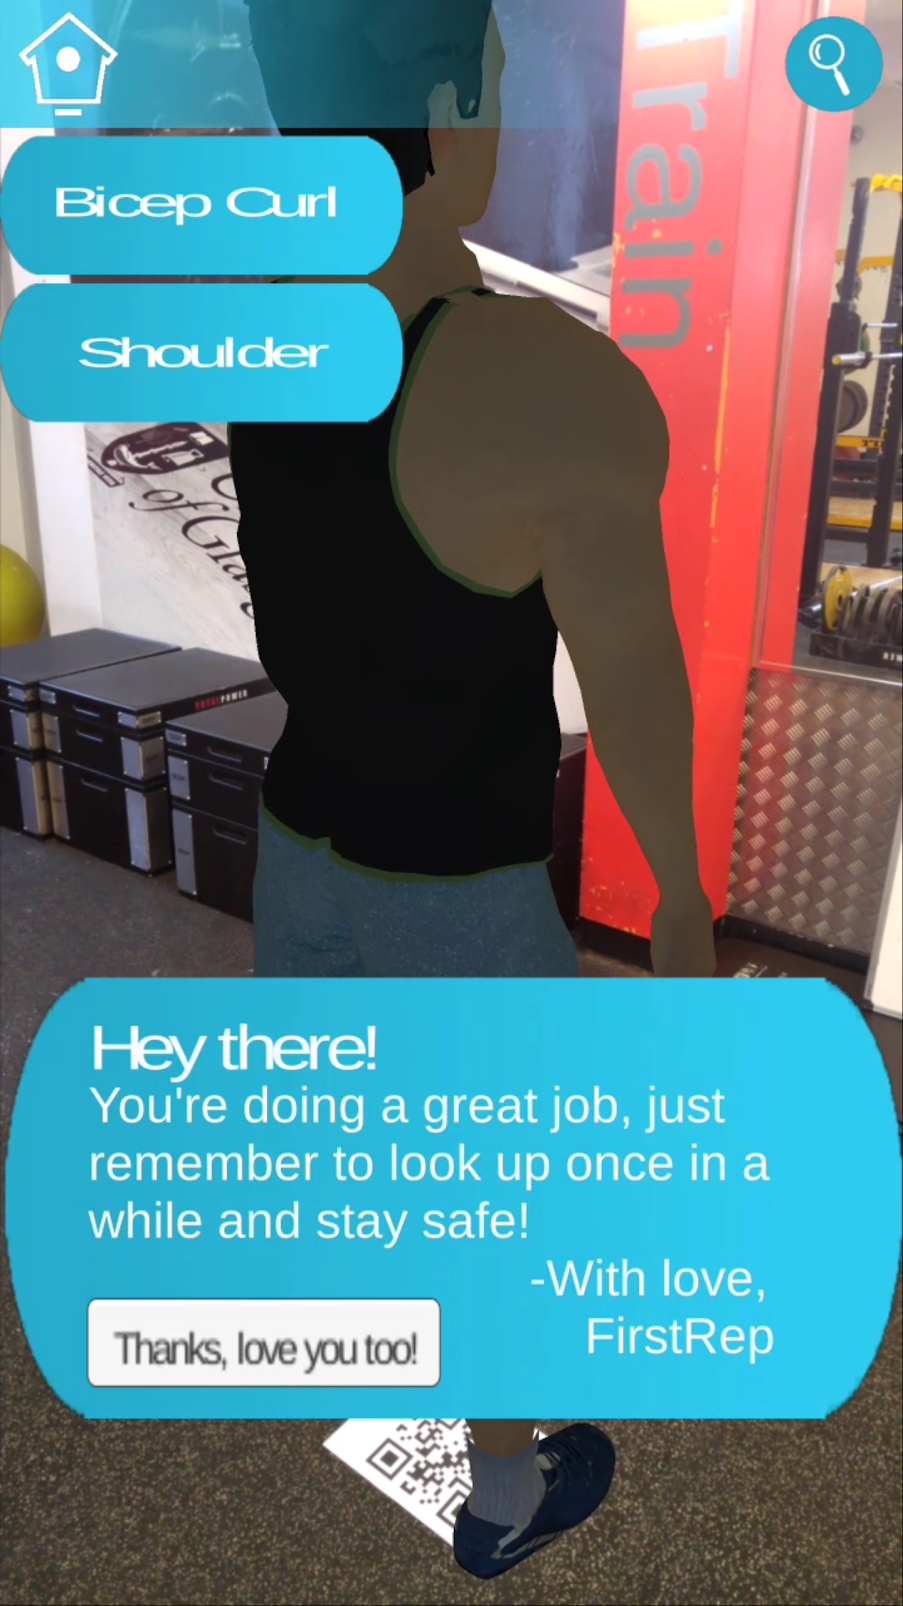
\includegraphics[height=8cm]{images/popup.png}
\caption{Screen shot of the warning popup} 
\label{fig:popup}
\end{figure}



%Include step by step instructions
The most significant change from the previous iteration was the implementation of the search view. During the trial, users were asked to try find exercises both by machine and muscle. No significant points of friction were identified and most feedback was positive, except for some suggested cosmetic changes such as making the home and back buttons more obvious (Table \ref{tbl:2ndtest}, Users C, D \& E). The initial fear that users may be confused by having animated exercises shown in both in AR view and in normal 2D view was completely dismissed. On the contrary, there was even demand to expand the 2D views with users suggesting adding step-by-step instructions to the 2D view as well as showing what equipment is needed to perform each exercise. The extra information could appear as cards at the bottom of the 2D view that the user can swipe up to scroll through the information on them.


\chapter{Evaluation}

%Evaluate based on initial requirements 
In accordance with Agile principles, the product has been evaluated throughout the lifetime of this project. Since the app is to be distributed in a two sided marketplace, both user trials in the gym and customer meetings have been carried out. After three iterations, two user trials and two customer meetings, the product is at a functional prototype stage and it is therefore time to review the product against the requirements set out earlier in Table \ref{acceptance_criteria}. In Table \ref{review} an evaluation of each of the requirements can be seen. Requirements II, III, V, VI \& VII have been fully satisfied and requirements I and IV are partially satisfied with future steps outlined. 

%Do I need to go through each of the requirements here, or is the summary enough ???

\begin{table}[]
\centering
\resizebox{\textwidth}{!}{%
\begin{tabular}{p{3cm}p{5cm}p{5cm}p{5cm}p{5cm}}
\textbf{Requirement Number} & \textbf{Requirement Text} & \textbf{Guiding Question} & \textbf{Acceptance Criteria} & \textbf{Result} \\\hline
I & Exploit situativity through location based interaction & Is the app usable in the gym? Is there utility from using the app in the gym as opposed to at home? & User feedback & Most users able to learn from the app (Table \ref{tbl:2ndtest}) Improvements necessary (option to change size of avatar) \\ \hline
II & Ensure the application is usable in any environment and with any brand of equipment & Does the app work anywhere and with any brand of equipment? & Test app with multiple manufactures/in multiple environment & QR code enables usage with in any environment/with any model \\\hline
III & Eliminate the need for an instructor to demonstrate an exercise & Can users use the app and gain knowledge by themselves? & User feedback & Most users able to learn from the all (Table \ref{tbl:2ndtest}) \\\hline
IV & Ensure that there are no issues with alignment or target recognition & Does the tracking work well? & User feedback & Somewhat satisfied, improvements necessary (option to change size of avatar) \\\hline
V & Create an easy to use on-screen graphical user interface & Do users understand how to use the app? & User feedback & Users like the interface (Tables \ref{survey_results} \& \ref{tbl:2ndtest}) \\\hline
VI & Avoid users from becoming fully immersed into the application & Is there any way to avoid users getting sucked into the app? & Observe users as they use the app & Popup is effective and users like it \\\hline
VII & Show theoretically perfect form and notify user of any dangers & Are users aware of any possible dangers? & User feedback & Pop up takes care of this, info screen also helps \\
\end{tabular}%
} 
\caption{A review of acceptance criteria for the project}
\label{review}
\end{table}

%What would I have done differently?
%More realistic testing
%Get user feedback sooner
%Start developing in the gym/lifesized markers sooner
Overall, the project has been quite successful. Even though progress was slow at the start, due to a constant steep learning curve, once all the tools were utilised in the proper way, the product really came together. One of the reoccurring problems throughout the project has been the tracking of and alignment with markers. Different types of markers in different sizes have been trialed but no combination seemed to work with life-sized avatars. The issue was that until the final user test, shrinking the size of the avatar was not seen an option because it was assumed that real-life size of the character was a fundamental requirement for the users. In the last trial, however, user feedback disproved this assumption and in fact, by shrinking the avatar the problem with alignment was solved. A quick prototype with significantly smaller avatars was developed and shown to some of the users who participated in the trials in an impromptu and informal setting. All agreed that shrinking the avatar greatly improved maneuverability and usability of the AR view. This experience goes to show that despite meeting with both the potential users and customers on several occasions, the project could have benefited from even more regular interaction with them. Interacting with stakeholders can be time consuming and requires a significant amount of effort however the benefits reaped are not to be underestimated. If trials in the university gym took place earlier on in the development process, any underlying assumptions regarding the scale of the markers and the avatar would have likely been dismissed much earlier, simplifying much of the development and removing confusion.

%Better software engineering
When creating a prototype, functionality is often favoured over code quality and process rigidity. As a prototype develops, spur of the moment decisions made in the past quickly accumulate into technical debt which can become a burden in the long run. This has also been the case for this project and therefore, a future improvement would be to introduce a number of process improvement techniques such as automated builds and more extensive testing. It was difficult to incorporate any automated testing into the project purely due to the fact that the problem domain, nor the tools used were largely unknown at the start of the project and therefore it was difficult to plan ahead and carry out any sort of test driven development. Currently the app is only a prototype and therefore a refactoring of some parts of the codebase may be in order to allow the app to scale in the future. For example, the available exercises are currently hard coded into the app whereas in the future these should be pulled dynamically from a database that is hosted on an external server. The mapping of state codes to different animations in the animation controller for the character will also need to be changed to accommodate future expansions. The current version of the animation controller was developed in the Unity GUI and has a number of states which are all interlinked. In the future, as the number of possible animations grows, the controller well need to be dynamically generated based on the exercises available in the database. This expansion is necessary both because the number of exercises will be unknown and because the growing complexity is hard to implement on a graphical interface. 

\section{Future Work}
%Next step
%Employ motion tracking to do the animations
There are a number of possible steps that can be taken to further develop the app. One of the most time consuming parts of development so far has been the creation of animations. Not only was there a steep learning curve at the beginning to learn how to create the animations but also the process itself was tedious, time consuming and produced unprofessional and unnatural looking animations. One possible way to simplify the process of creating animations would be to use motion capture. Blender, the software used to create animations, has an add on which enables the user to use their webcam to input track their movements and can used to record animations. The tool works based on the user identifying specific features on their body and mapping them to the rigged skeleton within Blender. Setting up the tool may initially require a significant amount of effort but in the long run it would greatly simplify and speed up the process of creating animations. If the project was to be carried out again, it would be advisable to use motion capture from the onset rather than attempting to create animations manually at first as this proved to be wasteful and in the end did not produce animations of professional fidelity. 

%Freemeium
%Can be a vehicle into other sports -yoga, climbing, swimming etc
Beyond the scope of this project, it could be an idea to monetise the app. Clearly, the current range of exercises is not enough to interest real users and therefore the set will have to be expanded. Any number of exercises could be included in the app however different users may have different opinions as to what exercises should be included and which should be left out. A possible way of solving this issue would be to split different exercises into packs and allow the user to pick a starting pack for free when they first use the app. Subsequent exercise packs could be downloaded, but at a small cost. By adopting a freemium model such as this the users are able to try out the app, decide if they like it and if so, buy more exercises. This approach not only generates profit but also allows the user to customise what exercises they see based on what activity they are most interested in. Possible packs could for example be a group of yoga poses, a selection for Olympic Weightlifting exercises or a set of dynamic workouts to do before sprint training. The possibilities as to what extension packs could be made available are endless and are only bounded by the ability to record the necessary animations and have them shown in a suitable environment. 


%Programing 
Alongside the core functionality of AR animations, the app could be extended much further to include a fitness tracker and workout programs. Users could download programs that would guide them, day-by-day, thorough what exercises they should be completing and how much volume (reps \& weight) they should be doing. Programs could target specific areas of improvement such as increasing the users maximum bench press or be more general programs, perhaps even inspired by celebrities such as "The Kim Kardashian Workout". Stretching the idea further, celebrities or firms could sponsor programs, generating another source of revenue for the app. The app would show the user the prescribed workout routines, changing them day by day and tracking their progress. Integrations with lifestyle apps such as MyFitnessPal could bring further utility to the user as the app would be able to reliably track the users calories output. 

%Customisation 
As users use the app more, they may very likely be interested in making the character look different to the default one provided. A phenomenon rooted in the Sims computer game, users are used to customising their avatars and the app should provide options to do so. Examples of customisations would be to make the character male or female, pick their skin tone, height, age and even provide a selection of outfits. By adapting the way the avatar looks, the users may develop a deeper relationship with the app and be likely to use it more. Default options for customising the character but other paid options may also be included or sponsors could pay to have their branded clothing appear as an option for the character to wear. Linking back to the previous suggestion about celebrity workouts, the character could morph into the given celebrity while you are following the program to make the experience more authentic. 


%Indoor navigation
Many of the initial users will likely be completely new to the gym and thus simply giving them the name of the equipment they are supposed to use will not give them much to go by. Users could benefit from having the application make use of indoor navigation and guide them straight to the correct equipment. Indoor navigation could be displayed on the AR view in the form of onscreen directions or simply as a large arrow pointing in the correct direction. There are a number of libraries that could be used to implement this functionality, such as TenDegrees, Steerpath or Wayfinder. TenDegrees and Wayfinder both provide plug-ins for Unity and Steerpath exposes an API to which the app could connect. The navigation system would probably need to involve the installation of a series of indoor bluetooth beacons to effectively locate the user, since GPS is unlikely to work inside a building with much precision. Indoor navigation would be nice to have however it is a difficult feature to implement and it would also require each individual gym to track exactly where each one of their machines is positioned in relation to the room In the short term it may be best to simply display the name of the machine and an accompanying image since this is significantly less difficult and serves a similar purpose. 
%TODO Cite
%http://www.tendegrees.net/
%http://touchez.co.uk/wp-content/uploads/2013/10/3D%20Wayfinder.pdf
%http://www.steerpath.com/indoor-positioning-api

% Other interfaces - google glass?
The application should be distributed not only on Android but also other platforms such as Windows phone and iOS. Since the app is built in Unity, it can be exported into each of the mentioned platforms, with minimal changes. In the future, the app could go further and be used on other platforms. Gyms could have a stock of a couple tablets which could be taken out by the user and carried around the gym for use. Alternatively, the app could run on a mixed reality device, such as the now abandoned Google Glass or similar wearable optic devices. 




\section{Conclusion}
Despite the wide ranging number of challenges that have had to be overcome over the duration of this project, the end result is overwhelmingly positive. The project has introduced a number of new technologies and tools and demonstrated the need for frequent and effective stakeholder interactions. The software engineering process followed during the project has stayed lean and Agile, adopting practices that made sense and discarding practices which would have added unnecessary bloat to the execution of the idea. An informed and measured academic approach was taken during the initial extraction of requirements and user opinion was taken into account at every step of the process. The app was created in an iterative fashion which helped shaped the end product and both answered questions and created new puzzles at every stage. In the end, all the efforts have come to fruition and what is left is a usable prototype of a Augmented Reality Gym app that not only serves as a proof of concept but also lays the foundation for future work. Clearly, steps must be taken for the app to be scalable however given the time, the limited experience within the field and the number of challenges overcome, this project has been a sensational success. 




%%%%%%%%%%%%%%%%
%              %
%  APPENDICES  %
%              %
%%%%%%%%%%%%%%%%
\begin{appendices}
\chapter{1 st User Testing Survey}
\label{survey}
\textbf{Question 1:} Gender \\
\textbf{Option(s):}    Male, Female, Prefer not to answer
\\
\\
\textbf{Question 2:} How often do you go to the gym? \\
\textbf{Option(s):}    Scale from 1 to 5 (Never - Every day)
\\
\\
\textbf{Question 3:} What do you think of the design? \\
\textbf{Option(s):}    Scale from 1 to 5 (Horrible - Awesome)
\\
\\
\textbf{Question 4:} How easy is the app to use? \\
\textbf{Option(s):}    Scale from 1 to 5 (Very Difficult - Very Easy)
\\
\\
\textbf{Question 5:} How likely would you be to use the app? 
\\
\textbf{Option(s):}    Scale from 1 to 5 (I wouldn't - I definitely)
\\
\\
\textbf{Question 6:} What is the best thing about the app? \\
\textbf{Option(s):}     Short Text Answer.
\\
\\
\textbf{Question 7:} What needs to be improved the most?? \\
\textbf{Option(s):}     Short Text Answer.
\\
\\
\textbf{Question 8:} Any further thoughts?? \\
\textbf{Option(s):}     Short Text Answer.


\chapter{2nd User Testing}
\label{survey2}
\textbf{Question 1:} How many days a week do you go to the gym? \\
\textbf{Option(s):} Scale from 0 to 7 (days/week)
\\
\\
\textbf{Question 2:} How did you find the design of the app? \\
\textbf{Option(s):} Short Text Answer
\\
\\
\textbf{Question 3:} How easy was navigating around the app? \\
\textbf{Option(s):} Short Text Answer
\\
\\
\textbf{Question 4:} How easy/difficult was using the augmented reality view? \\
\textbf{Option(s):} Short Text Answer
\\
\\
\textbf{Question 5:} Would you be able to learn a new exercise based on the animations? \\
\textbf{Option(s):} Short Text Answer
\\
\\
\textbf{Question 6:} What would you change about the app? \\
\textbf{Option(s):} Short Text Answer
\\
\\
\textbf{Question 7:} What other features would you like to see? \\
\textbf{Option(s):} Short Text Answer
\\
\\
\textbf{Question 8:} What was your favorite feature of the app? \\
\textbf{Option(s):} Short Text Answer
\\
\\
\textbf{Question 9:} Would you recommend the app to a friend? \\
\textbf{Option(s):} Short Text Answer	

\end{appendices}

%%%%%%%%%%%%%%%%%%%%
%   BIBLIOGRAPHY   %
%%%%%%%%%%%%%%%%%%%%

\bibliographystyle{plain}
\bibliography{bib}

\end{document}
